



%
%
% ***********************************************************************
%
%

%  Getting_started 2



\chapter{Getting  started 2D}


In this  second  example  we  will  refer  to  the  \textbf{Tutorial 4} (Si n-Mosfet) that you  can  find  in  the  \textit{Tutorials}  directory.



\section*{Step 1: Modeling the device}

Again, as a first step, we have to model the device. 

We'll see in some details how to design and mesh a mosfet device with GMSH.


\begin{itemize}
\item 
In the  GMSH script  \textit{mosfet.geo} , several variables are  defined and given a value in this way:                                                 \end{itemize}


\begin{verbatim}
lsub=0.03;
lacc=0.002;
lct=0.0005;
lg=0.0015;
lh=0.01;
lc=0.0005;
\end{verbatim}

these variables are used in the script to assign proper values to the \textbf{mesh characteristic lengh} of the defined Points 

\begin{verbatim}
Lg_2 = 0.0375;
d = 0.01;
Ls = 0.1;
h = 0.25;
b = 0.0025;
o = 0.005;

xd = Lg_2 + d;
xd2 = Lg_2 + d / 2;
xmax = xd + Ls - d;
\end{verbatim}
These other convenient variables are used to parametrize the most relevant geometrical features, such as channel length, oxide thickness,  and  so on. 


\begin{verbatim}
Point(1) = {0, -h, 0, lsub};
Point(2) = {0, 0, 0, lc};
Point(3) = {xmax,-h,0.0,lsub};
Point(4) = {-xmax,-h,0.0,lsub};
Point(5) = {xmax,0,0.0,lh};
Point(6) = {-xmax,0,0.0,lh};
..........................
Line(1) = {4,1};
Line(2) = {3,13};
Line(6) = {4,14};
Line(7) = {10,9};
Line(8) = {12,2};
Line(9) = {8,7};
Line(10) = {11,8};
Line(11) = {9,12};
Line(13) = {7,6};
..........................
\end{verbatim}

\begin{itemize}
\item 
Geometrical \textbf{Points} and \textbf{Lines} are  defined to design the device  structure; the  fourth parameter in \textbf{Point} assignement is  the   characteristic length associated to that point: this  is  an  essential feature to control the  mesh density and refine it where  necessary (usually n the channel region).     \end{itemize}

 

\begin{verbatim}
Line Loop(40) = {28,2,-34,33,8,29,-31,-30,-6,1};
Plane Surface(41) = {40};
..........................
\end{verbatim}
\begin{itemize}
\item 
Definition of a surface: first a \textbf{line loop} is composed, listing all the  lines constituting the  boundary of the surface; then this  line  loop is  assigned to a  \textbf{Plane Surface} object (this  procedure can be alternatively performed throgh the  graphical interface).                       \end{itemize}                                                                                                                                                                                                                             



\begin{verbatim}
Physical Surface(1) = {41}; // n-Si
Physical Surface(2) = {44,47}; // n+-Si
Physical Surface(3) = {46}; // SiO2
\end{verbatim}
\begin{itemize}
\item 
Definition of  the \textbf{Physical surfaces} : each of them is composed by one or more geometrical \textbf{Plane Surface}. For example, \textbf{Physical surface} 2 comprises the two separated contact regions, while \textbf{Physical surface} 3 corresponds to the  oxide  region.

The  \textbf{Physical surfaces} are the 2D Physical regions of  the  mesh and will  be  assigned to the related \TiberCAD regions through the keyword \textit{mesh\_regions}  (see   Step  )                                                                                                                   \end{itemize}                                                                   


\begin{verbatim}
Physical Line(1) = {13}; // source
Physical Line(2) = {39,38}; // gate
Physical Line(3) = {19}; // drain
\end{verbatim}
\begin{itemize}
\item 
Definition of the  \textbf{Phisical Lines}: In this 2D simulation, 1D physical regions are used to carry information about boundary condition regions. In  other word, each \textbf{Phisical Line} corresponds to a boundary condition (a contact in the case of a driftdiffusion calculation): thus Physical Line 1 refers to source contact, P.L. 2 to gate contact, P.L. 3 to drain contact.
The numerical identifications of these \textbf{Phisical Lines} will be  asigned to \TiberCAD \textbf{BC regions} by means of the \textit{BC\_reg\_numb} instruction.
\end{itemize}

In fig.  \ref{geo}  the  obtained  geometrical  model is  shown.


\begin{figure}
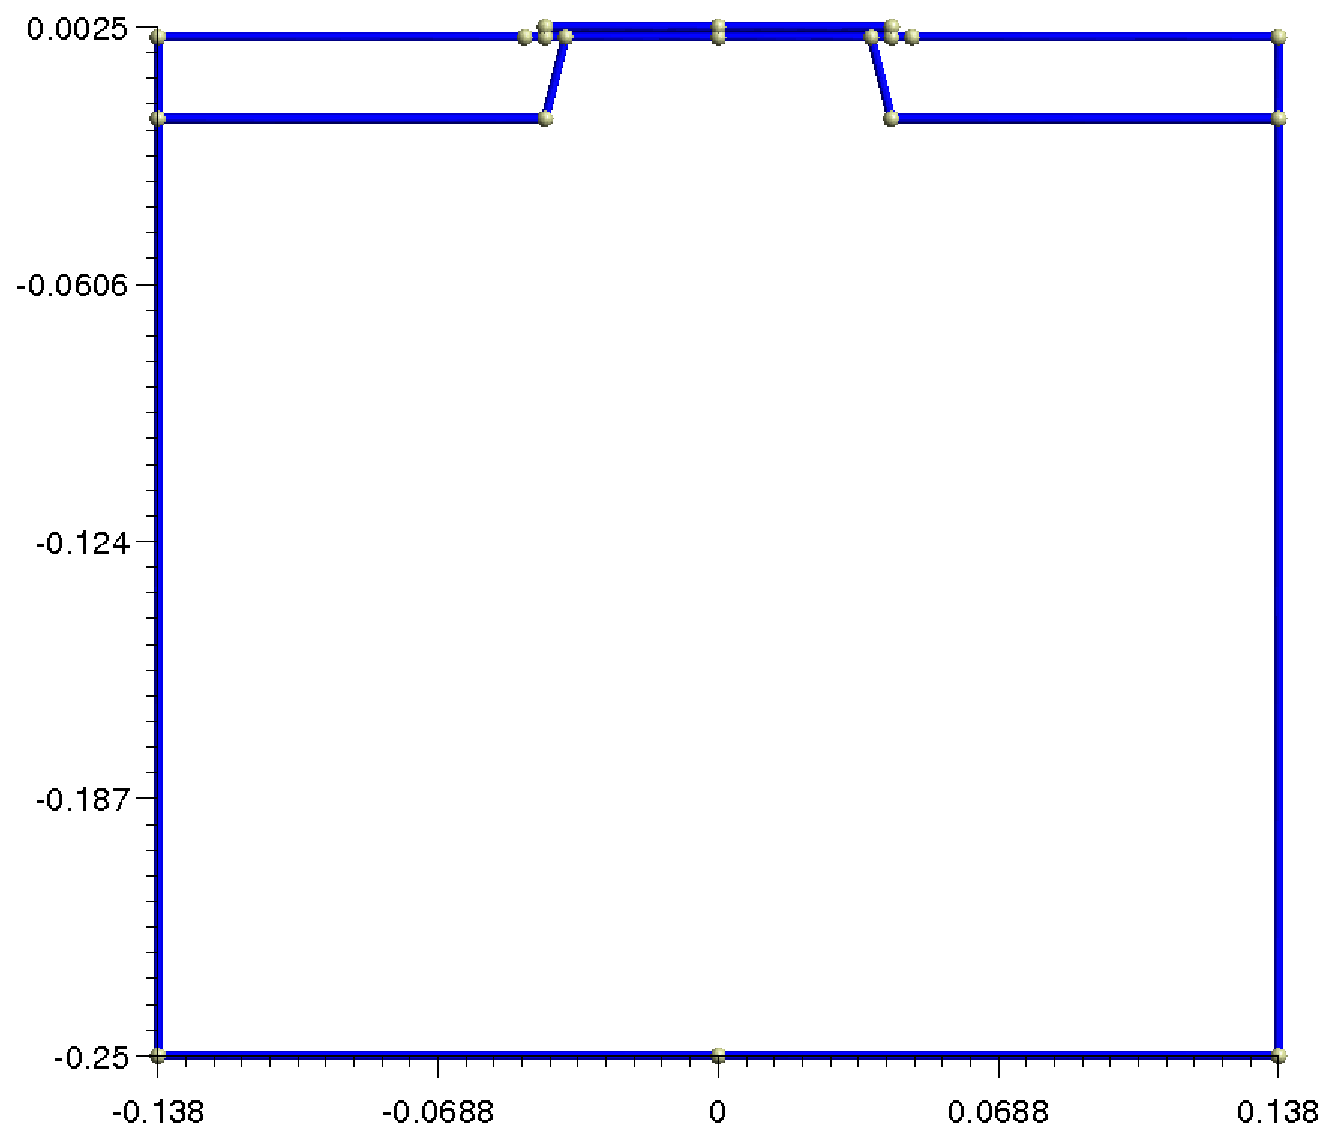
\includegraphics[width=8cm]{./figures/geomosfet}

%\centerline{
\psfig{figure=geomosfet.ps, angle = 270,width=9cm }}
\caption{Geometrical structure as  defined by GMSH modeller}
\label{geo}
\end{figure}
 


\section*{Step 2: Meshing the device}

The \textit{.geo} script file with the geometrical description can be run in GMSH, to display the modelled device and to mesh it through the GMSH graphical interface (see fig. \ref{meshmos}).
Alternatively, a \textit{non-interactive} mode is also available in GMSH, without graphical user interface. For example, to mesh this 2D tutorial in non-interactive mode, just type:

\textit{gmsh mosfet.geo  -2 -o mosfet.msh }

\begin{figure}
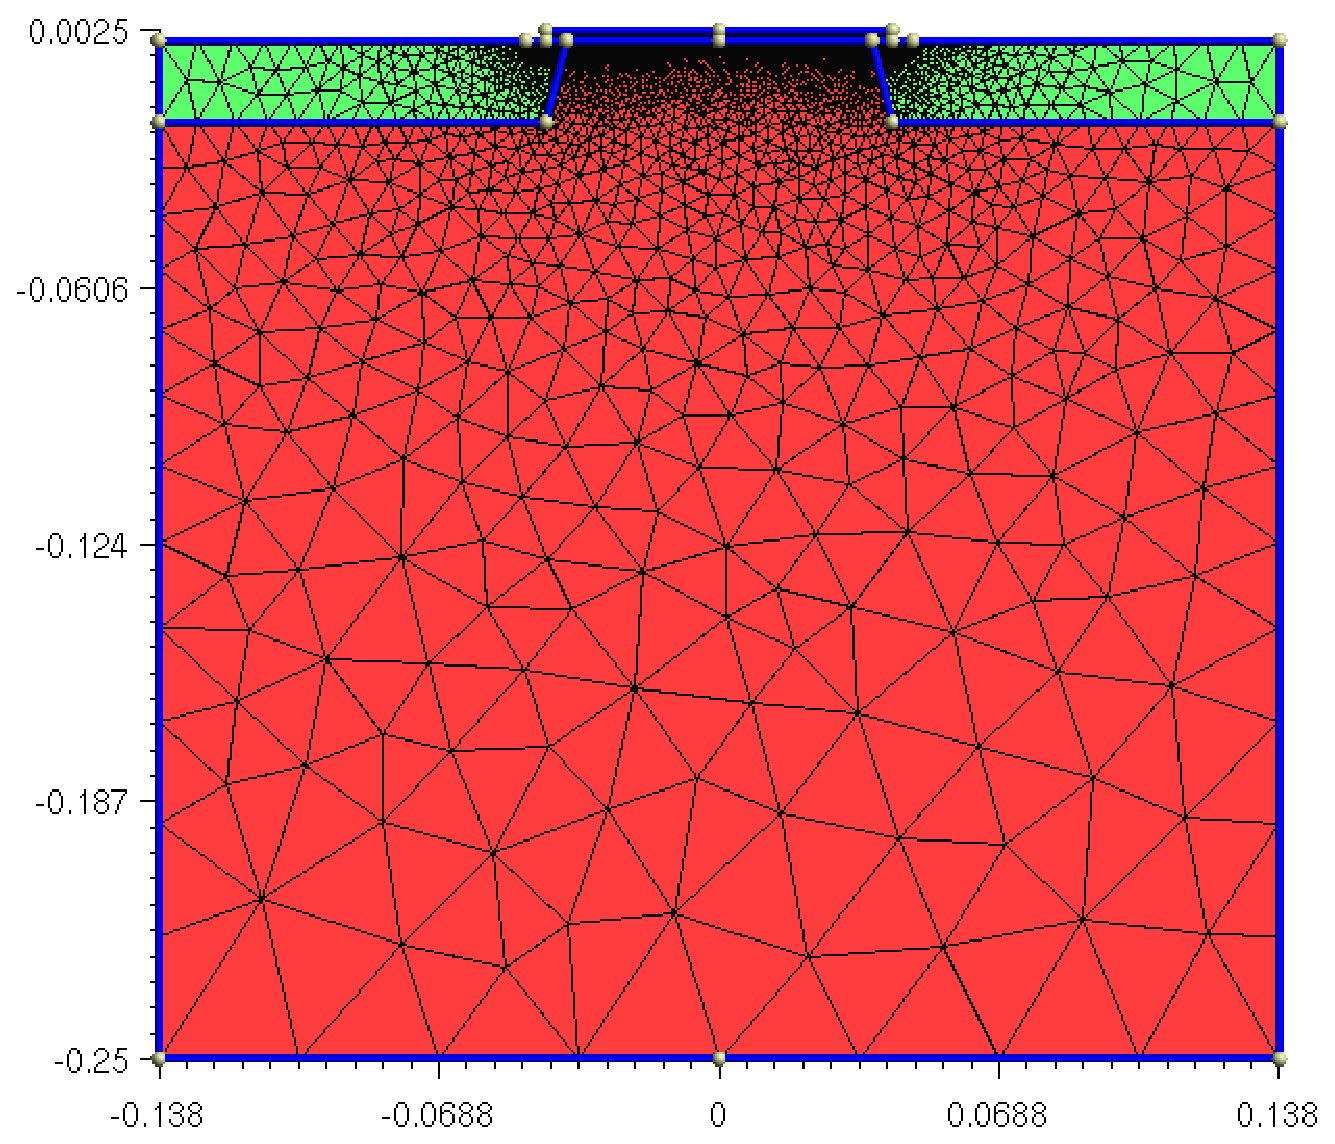
\includegraphics[width=8cm]{./figures/meshmosfet}

\caption{2D Mesh for the mosfet device obtained with   GMSH }
\label{meshmos}
\end{figure}




\section*{Step 3: TiberCAD  Input file  }

Now we have to write down the \TiberCAD \textbf{input file} (see \textit{mosfet.tib} in  the  Tutorials).


\subsection* {1 - Definition of Device Regions}

Three  \TiberCAD regions are  defined: to each of them, one  mesh\_region is  associated, that is the Phisical Surfaces  \textbf{1, 2} and  \textbf{3} defined in  Step 1. However, in general more than one  mesh\_region can be  associate to a single \TiberCAD region, if this is convenient.

\begin{verbatim}
 Region substrate 
   {
     mesh_regions = 1
     material = Si
     doping = 1e18 doping_type = acceptor
   }
   
   Region contact
   {
     mesh_regions = 2
     material = Si
     doping = 5e19 doping_type = donor
   }

   Region oxide
   {
     mesh_regions = 3
     material = SiO2
  
   }

\end{verbatim}


\subsection* {2 - Definition of Simulation}

Now we define the \textbf{Simulation} \textit{dd}: it belongs to  the class \textbf{driftdiffusion}

\begin{verbatim}
   model driftdiffusion
  { 
              
    options
    {
     simulation_name = dd
     physical_regions = all
    }


\end{verbatim}

We declare two \textbf{driftdiffusion physical models}:
 the  first defines a   \textit{srh} \textbf{recombination}  model (see \ref{dd:recomb_models}); the  second 
defines a \textit{field-dependent} \textbf{mobility} model for  electrons which implements a \textit{doping  dependence} for the \textbf{low-field  mobility} (see \ref{dd:mobility_models}).

% respectively about \textbf{mobility} (\textit{field\_dependent}) and  \textbf{recombination} (\textit{srh});  see  the reference manual  for  the  details \ref{dd:recomb_models}, \ref{dd:mobility_models}

\begin{verbatim}

    physical_model recombination
    {
      model = srh
    }

    physical_model electron_mobility
    {

      model = field_dependent
      low_field_model = doping_dependent   

    }



\end{verbatim}

\subsection* {3 - Definition of Boundary Conditions}
The source, drain  and gate contacts of the Mosfet device  are defined as \textbf{Boundary conditions regions} (\textit{BC\_Region source , BC\_Region drain, BC\_Region gate }) in the following way:

\begin{verbatim}
    BC_Region gate
      {
        BC_reg_numb = 2
        type = schottk
        barrier_height = 3.0
        voltage = @Vg[0.0]
      }

      BC_Region source
      {
        BC_reg_numb = 1
        type = ohmic
        voltage = 0.0
      }
 
      BC_Region drain
      {
        BC_reg_numb = 3
        type = ohmic
        voltage = @Vd[0.5]
      }


\end{verbatim}

To each of the  \textbf{BC regions}, one \textit{BC\_reg\_numb} is  assigned,  that  is  one  of the Physical Lines \textbf{1,2, 3} defined in \textbf{Step 1}, which represent the contact regions.

Note that, while \textit{source} and \textit{drain} are defined as \textit{type= ohmic},  \textit{gate} \textbf{BC region} is defined as \textit{type = schottky};
\textit{barrier\_height = 3.0} specifes the metal/oxide interface barrier and depends on the contact metal workfunction.

Drain voltage is defined as \textit{@Vd[0.5]} and  gate voltage as \textit{@Vg[0.0]}. This specifies that the value of the voltage will be  determined at each moment of the simulation, by the value of the two variables \textit{Vd} and \textit{Vg}, which will be assigned in the \textbf{sweep}  definition. 

 
\subsection* {4 - Definition of Simulation parameters}

Two sweeps are requested for this simulation, that is an external loop on \textit{Vg} (the gate voltage) and an internal loop on \textit{Vd} (the drain voltage) for each value of \textit{Vg}; in this way, the IV drain characteristics for a series of gate biases are obtained in output.

\begin{verbatim}
    sweep_1
  {
    simulation = dd
    variable = Vd
    start = 0.0
    stop = 2.0 #0.1
    steps = 200  #200 #1
 #   plot_data = true
  }

  sweep_2
  {
    variable = Vg
    start = -0.1
    stop = 0.5
    steps = 6
    simulation = sweep_1
    #simulation = driftdiffusion
  }


\end{verbatim}


\subsection* {5 - Definition of Execution parameters}

In the \textbf{Simulation} section , we decide    the  simulation dimension  (\textit{dimension = 2}), then \textit{which} simulations to perform
 and in which \textit{order}; we set
\textit{solve = sweep\_2}, to execute the external  gate  voltage sweep \textit{sweep\_2} which in  its  turn  call the sweep \textit{sweep\_1}  where drain current is  calculated for all the  chosen  drain voltage  steps by running   \textit{dd} \textbf{simulation}.

\begin{verbatim}
$Simulation
{
   meshfile = mosfet.msh
  dimension = 2
  temperature = 300
  solve = sweep_2 
  resultpath = output_IV_char 
  output_format = vtk
  plot = (Ec, Ev, QFermi_e, QFermi_h, eDensity, hDensity, eCurrent, hCurrent, 
          NetRecombination, EField, ElPotential, ContactCurrents)
}

\end{verbatim}

Output files with conduction and valence band profiles, quasi-fermi levels, electron and hole  density, recombination, electric field and potential (\textit{plot = Ec,Ev,....}.) will be  generated, together (\textit{ContactCurrents}) with  a file with  all the calculated values of the drain current at the contacts for each  gate bias  step  (the IV characteristics).

\section*{Step 4: Run TiberCAD}

Now we can run TiberCAD:

\texttt{tibercad  mosfet.tib}


\vspace{0.5cm}
The generated \textbf{Output} files are:

\textbf{driftdiffusion\_materials.vtk}:  information about the material regions of the device.

\textbf{driftdiffusion\_nodal.vtk}   output for the nodal quantities which have been calculated, e.g. conduction and valence bands, (quasi)fermi levels, electron and hole density and mobility.

\textbf{driftdiffusion\_elemental.vtk}  output for the elemental  quantities (e.g. electric field, current density).


\textbf{sweep\_2\_driftdiffusion\_Vg\_0.000\_Vd.dat}  and  similar for  all the  \textit{Vg}  steps: drain current characteristics for each \textit{Vg} bias.






